\pagestyle{fancy}
\chapter{Specification about experimental methods}
\section{Chemicals}
            \label{appendixresists}
           
            \begin{figure}[H]
            \centering
            \chemfig{CH_3-[:270]C(=[:180]CH_2)(-[:270]C(=[:0]O)(-[:270]O(-[:315]CH_3)))}
            \caption{Chemical structure of MMA, PMMA is a polymer made of this monomer}
            \label{PMMA}
            \end{figure}
                                   
            \begin{figure}[H]
                \centering
                \chemfig{-[:-30](-[:30]-[:-30](-[:30])(=[:270]O))(-[:270])}
                \caption{Chemical structure of MethylIsoButylKetone (MIBK)}
                \label{MIBK}
            \end{figure}
            
\section{EBL schematics}
\label{appendixEBL}
\begin{figure}[H]
                    \centering
                    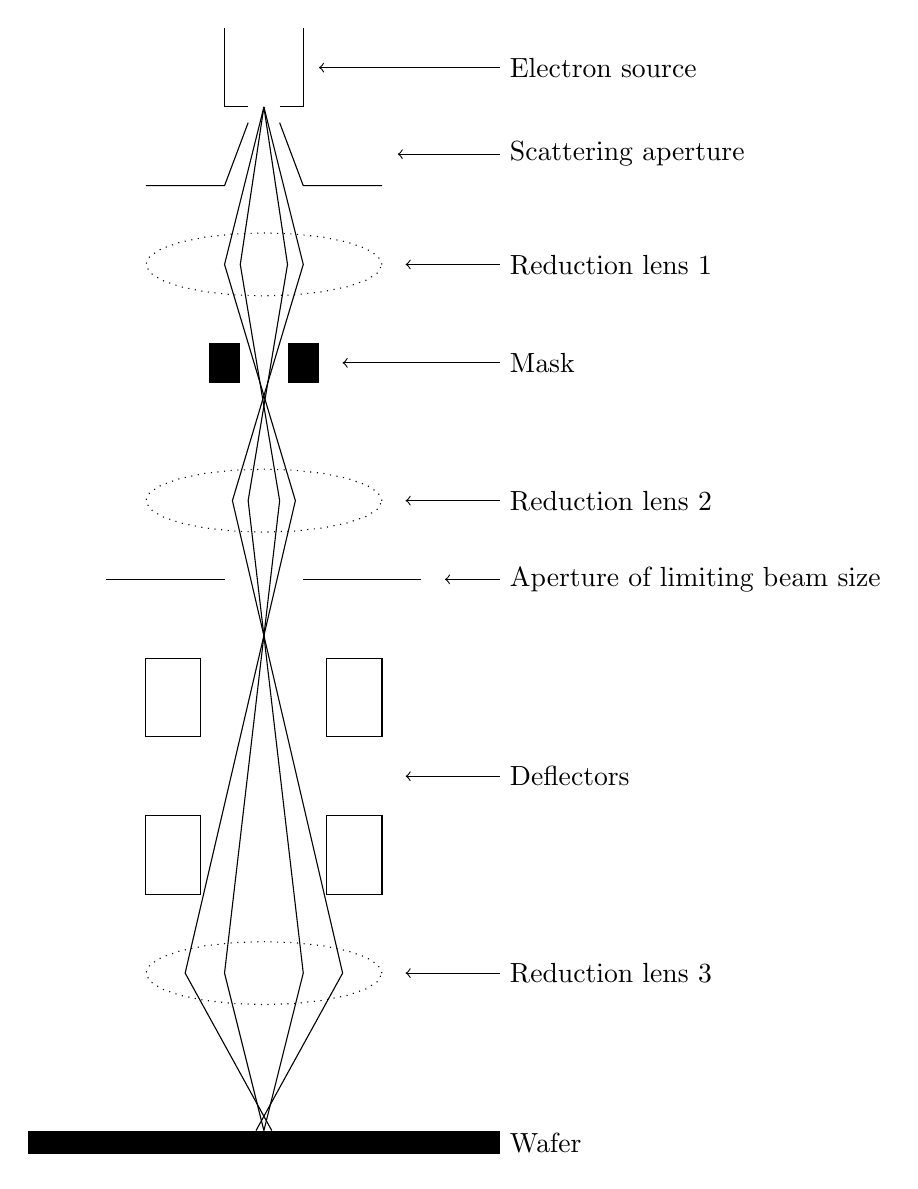
\begin{tikzpicture}
                    \draw (4.5,20)--(4.5,19)--(4.8,19);
                    \draw (5.2,19)--(5.5,19)--(5.5,20);
                    \draw [<-] (5.7,19.5)--(8,19.5);
                    \draw (8,19.5)node[right]{Electron source};
                    
                    \draw (3.5,18)--(4.5,18)--(4.8,18.8);
                    \draw (6.5,18)--(5.5,18)--(5.2,18.8);
                    \draw [<-] (6.7,18.4)--(8,18.4);
                    \draw (8,18.4)node[right]{Scattering aperture};
                    
                    \draw [dotted] [domain=0:360] plot({1.5*cos(\x)+5},{0.4*sin(\x)+17)});
                    \draw [<-] (6.8,17)--(8,17);
                    \draw (8,17)node[right]{Reduction lens 1};
                    
                    \fill (4.7,16)--(4.7,15.5)--(4.3,15.5)--(4.3,16)--cycle;
                    \fill (5.3,16)--(5.3,15.5)--(5.7,15.5)--(5.7,16)--cycle;
                    \draw [<-] (6,15.75)--(8,15.75);
                    \draw (8,15.75)node[right]{Mask};
                    
                    \draw [dotted] [domain=0:360] plot({1.5*cos(\x)+5},{0.4*sin(\x)+14)});
                    \draw [<-] (6.8,14)--(8,14);
                    \draw (8,14)node[right]{Reduction lens 2};
                    
                    \draw (3,13)--(4.5,13);
                    \draw (7,13)--(5.5,13);
                    \draw [<-] (7.3,13)--(8,13);
                    \draw (8,13) node[right]{Aperture of limiting beam size};
                    
                    \draw (3.5,12)--(4.2,12)--(4.2,11)--(3.5,11)--cycle;
                    \draw (6.5,12)--(5.8,12)--(5.8,11)--(6.5,11)--cycle;
                    \draw (3.5,10)--(4.2,10)--(4.2,9)--(3.5,9)--cycle;
                    \draw (6.5,10)--(5.8,10)--(5.8,9)--(6.5,9)--cycle;
                    \draw [<-](6.8,10.5)--(8,10.5);
                    \draw (8,10.5)node[right]{Deflectors};
                                                            
                    \draw [dotted] [domain=0:360] plot({1.5*cos(\x)+5},{0.4*sin(\x)+8)});
                    \draw [<-] (6.8,8)--(8,8);
                    \draw (8,8)node[right]{Reduction lens 3};
                    
                    \fill (2,6)--(8,6)--(8,5.7)--(2,5.7)--cycle;
                    \draw (8,5.85) node[right]{Wafer};
                    
                    \draw (5,19)--(4.5,17)--(5.4,14)--(4,8)--(5.1,6);
                    \draw (5,19)--(5.5,17)--(4.6,14)--(6,8)--(4.9,6);
                    \draw (5,19)--(4.7,17)--(5.2,14)--(4.5,8)--(5,6);
                    \draw (5,19)--(5.3,17)--(4.8,14)--(5.5,8)--(5,6);
                    \end{tikzpicture}
                    \caption{Simplified EBL functional diagram}
                    \label{EBLschema}
            \end{figure}
 
\chapter{Parameters table of the samples}
\label{parametertable}

\begin{tabular}{|c|c|c|c|c|c|}

        \hline
        \textsc{Test n\textdegree}&\textsc{Strong}&\textsc{Plasma}&\textsc{Regular}&\textsc{Comment}\\
        &\textsc{Oxidation}&&\textsc{Oxidation}&\\
        \hline
        Test 10&  &&&Failed EBL\\
        \hline
        Test 11&  &&&Failed EBL\\
        \hline
        Test 12&No&No&No&Clean contact reference\\
        \hline
        Test 13.i&Yes&10 min&No&Several positions\\
        \hline
        Test 14.i&Yes&20 min&No&Several positions\\
        \hline
        Test 15&Yes&No&No&Strong Oxidation reference\\
        \hline
        Test 16&No&No&Yes&Reference Sample Test 17\\
        \hline
        Test 17&Yes&10 min&Yes&Resist burned\\
        \hline
        Test 18&Yes&10 min&Yes&Resist burned\\
        \hline
        Test 19&No&No&Yes&Reference Sample Test 18\\
        \hline
        Test 20&Yes&10 min&Yes&Resist burned\\
        \hline
        Test 21&No&No&Yes&Reference Sample Test 20\\
        \hline
        Test 22&Yes&5 min&No&\\
        \hline
        Test 23&Yes&2 min 30s&No&\\
        \hline
        Test 24&Yes&10 min&Yes&Etched the wafer\\
        \hline
        Test 25&No&No&Yes&Reference Sample Test 24\\
        \hline
        Test 26&Yes&2 min&Yes&\\
        \hline
        Test 27&No&No&Yes&Reference sample Test 26\\
        \hline
        \end{tabular}
\vspace{0.5cm}

\noindent Parameters : 
\begin{itemize}
    \item Pad dimensions : 150$\times$150$\mu m$
    \item Lead length : 96$\mu m$
    \item Strong Oxidation = 10 min under a pressure of 200 mbar of O$_2$
    \item Regular Oxidation = 2 min under a pressure of 2 mbar of O$_2$
    \item Plasma = Pressure of Ar of 4.10$^{-4}$ mbar, Power=40mA, Extraction=-0.8kV\footnote{Lowered to -0.25kV starting from Test 22}, Ion Energy=1.5kV 
\end{itemize}

\chapter{Gantt Diagramm}

\begin{ganttchart}[hgrid, vgrid, y unit title=.6cm]{1}{13}
\gantttitle{2015}{13} \\
\gantttitle{May}{2}
\gantttitle{June}{4}
\gantttitle{July}{4}
\gantttitle{August}{3}\\
\gantttitle{Weeks}{13}\\
\gantttitlelist{1,...,13}{1}\\
\ganttbar{Subject and integration}{1}{2}\\
\ganttbar[bar/.append style={fill=black}]{Learning about tools}{3}{4}\\
\ganttbar[bar/.append style={fill=yellow}]{Literature}{2}{3}
\ganttbar[bar/.append style={fill=yellow}]{}{6}{7}
\ganttbar[bar/.append style={fill=yellow}]{}{9}{10}
\ganttbar[bar/.append style={fill=yellow}]{}{13}{13}\\
\ganttbar[bar/.append style={fill=red}]{Fabrication of structures}{4}{8}
\ganttbar[bar/.append style={fill=red}]{}{11}{12}\\
\ganttbar[bar/.append style={fill=green}]{300K measurements}{4}{8}
\ganttbar[bar/.append style={fill=green}]{}{11}{12}\\
\ganttbar[bar/.append style={fill=blue}]{Low temperature measurements}{9}{12}\\
\ganttmilestone{Cleanroom maintenance}{9}\\
\ganttmilestone{Oxygen cleaning}{10}\\
\ganttbar{Report redaction}{13}{13}
\end{ganttchart}

%images SEM ???


%\chapter{Matlab programs}

%\section{}
